\documentclass{article}

\title{Program Language and Design Assignment 5}
\author{Divij Singh}
\date{30/11/18}
\usepackage{graphicx}


\begin{document}

	\maketitle
	A simple feature enhancement for this would be the introduction of Object Oriented Principles.\\ \\
Put simply, the programmer should be able to compartmentalise blocks of code into 'objects', and tag them with a label. They can then call these blocks via the label, rather than have to re-write the entire block of code. To give a visual idea:\\ \\


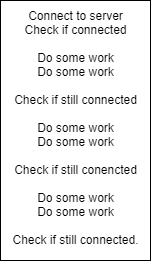
\includegraphics{normal.png}

Here, there is original design. There is a single block of code, with repeated lines to check the server connection. Upon breaking it up into objects, however: \\

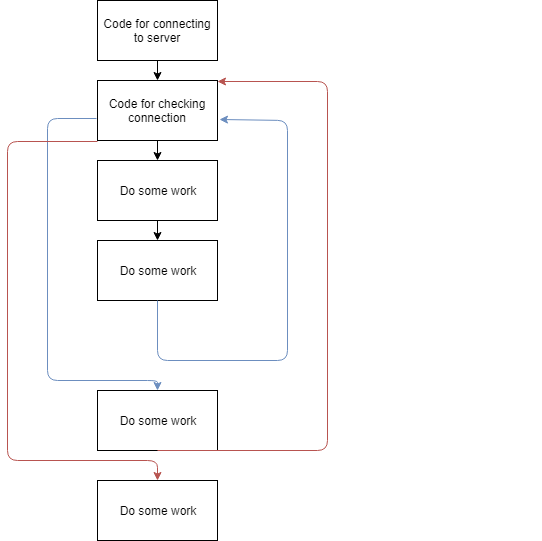
\includegraphics[scale=0.8]{suggested.png}

The server connection check block is written once, and then merely called upon when needed.
\end{document}